\section{Improve the memory pipeline}
\label{sec:memory_pipeline_improvements}

There are two major potential improvements in the current pipeline that remain

\subsection{Store image buffers directly in GPU accessable memory}
The first potential improvement is to store the image buffers directly in GPU accessable memory, as it will remove the redundant first copy operation in Figure \ref{fig:pipeline_current}.
This improvement relies on \lucid changing their \gls{api} as the current \gls{api} does not support this and the source code is not available.
I have communicated with a \lucid employee over email, and he said that they will looking into adding this feature in the future \cite{martensRe17896Use2023}.
After some discussion on how this could be implemented we came to the conclusion that a clean way would be have an optional argument that would make the \gls{api} use Pinned Memory instead of regular Pageable host memory.
Another more modular approach I sugessted is to allow the user to pass in pointers to preallocated memory where the images should be stored, enabling the use of any tyupe of \gls{cpu} accessable memory.
As of today the engenering department at \lucid has not yes implemented any of these features, but hopefully they will be implemented in the future.

\begin{figure}[H]
    \centering
    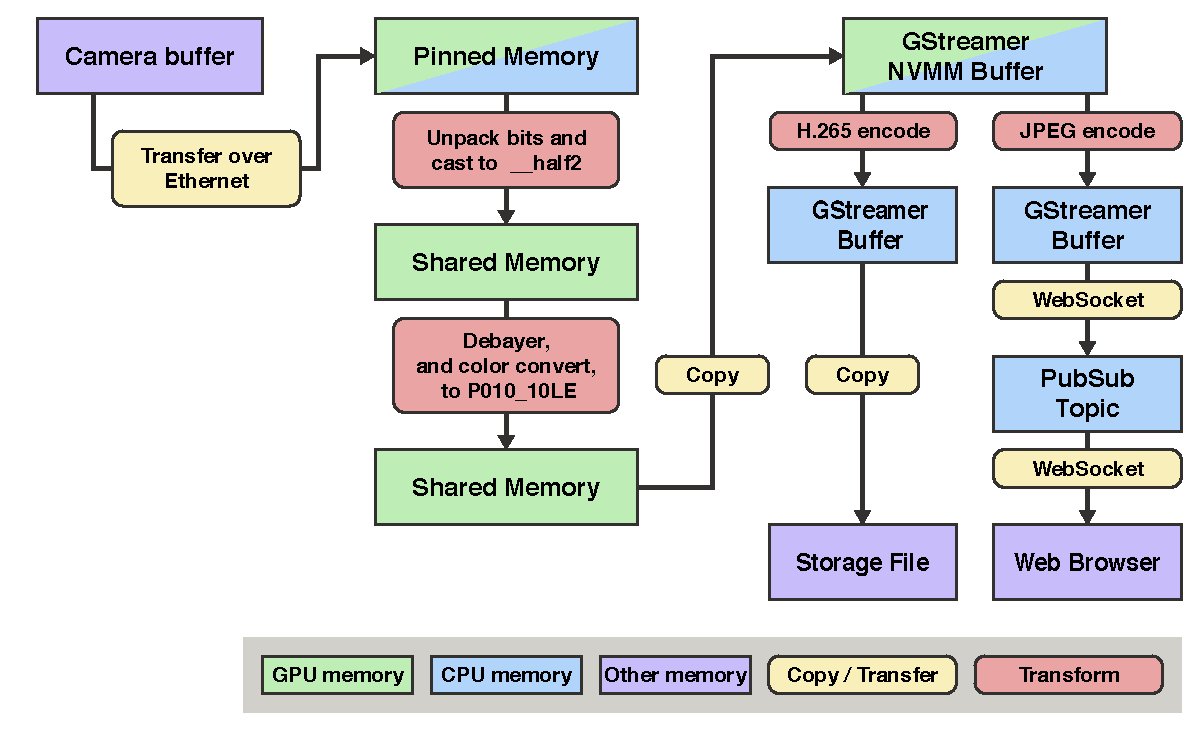
\includegraphics[width=\textwidth]{figures/memory_pipeline/optimal.pdf}
    \caption{Overview of an improved pipeline compared to Figure \ref{fig:pipeline_current}.}
    \label{fig:pipeline_optimal}
\end{figure}

\subsection{Better integration with GStreamer}
Many limitations of \gls{pygo} seem to be addressed by the \gls{pyds} library.

It serves as a wrapper for NVIDIA's \gls{ds} \gls{sdk}, which is a framework for accelerated \gls{ai} applications \cite{nvidiaDeepStreamSDK2016}.
By leveraging \gls{pybind11}, \gls{pyds} extends the functionality of \gls{pygo} with custom bindings to \gls{gstreamer} related functions \cite{nvidiaaiiotReleasesNVIDIAAIIOTDeepstream}.
The library offers a comprehensive tutorial on expanding its capabilities through the creation of custom functions and bindings \cite[\textit{bindings/BINDINGSGUIDE.md}]{nvidiaaiiotReleasesNVIDIAAIIOTDeepstream}.
\gls{pyds} should enable the createtion \glspl{nvmmbuffer} in \py using \code{NvBufSurfaceCreate} \cite{nvidiaNvBufSurfaceCreateDeepstreamDeepstream2023}\cite{babukrCreatingGstBuffersUsing2021}.
Consequently, this would eliminate two unnecessary copy operations by enabling a direct transfer from shared memory to a \gls{nvmmbuffer}, as depicted in Figure \ref{fig:pipeline_optimal}.

It is worth noting that this can be considered overoptimization, as memory bandwidth is far from being the bottleneck in the current pipeline.
